\section{RNA-seq analyses of blood-induced changes in gene expression in the mosquito vector species, \Aea\ \cite{Bonizzoni2011}}

\begin{figure}[hp]
\centering
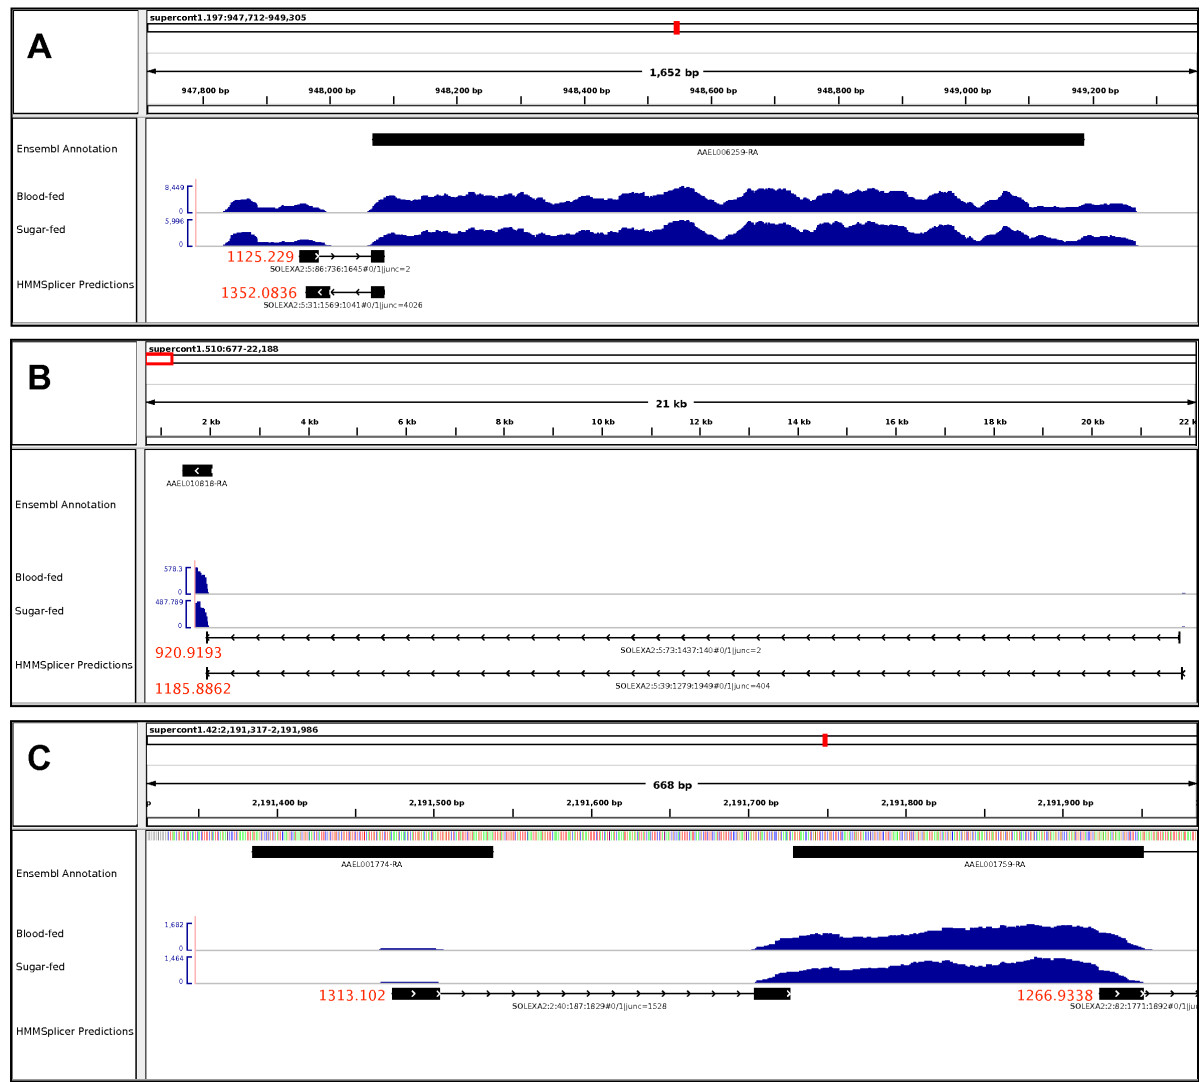
\includegraphics[width=.95\textwidth]{figures/figs/aedesHMMsplice.jpg}

\caption[Examples of amendments to the \Aa\ annotation supported by HMMSplicer results]{\sf \textbf{Examples of amendments to the \Aa\ annotation supported by HMMSplicer results:} Black bars in the top tracks represent the current gene annotations. Blue histograms in the second track represent the non-normalized coverage of RNA-seq reads at each position. The range of the histogram values shown in each view is depicted on the labeled y-axis of each RNA-seq track. Black boxes in the lower track represent splice-site predictions based on the RNA-seq reads using HMMSplicer determined in this study. Each function has a unique identifier listed below and its HMMSplicer score is listed in red. If multiple reads support a single junction, "junc = x" lists the number of supporting reads. This information provides evidence to link two islands of transcription as a single transcription event, therefore, exons of a common mRNA. All predicted junctions shown here also are supported by EST alignments. Genes are (A) AAEL006259; (B) AAEL010818; and (C) AAEL001774 and AAEL001759.

Excerpted from \cite{Bonizzoni2011}}
\label{fig:aedesHMMsplice}
\end{figure}

\begin{figure}[hp]
\centering
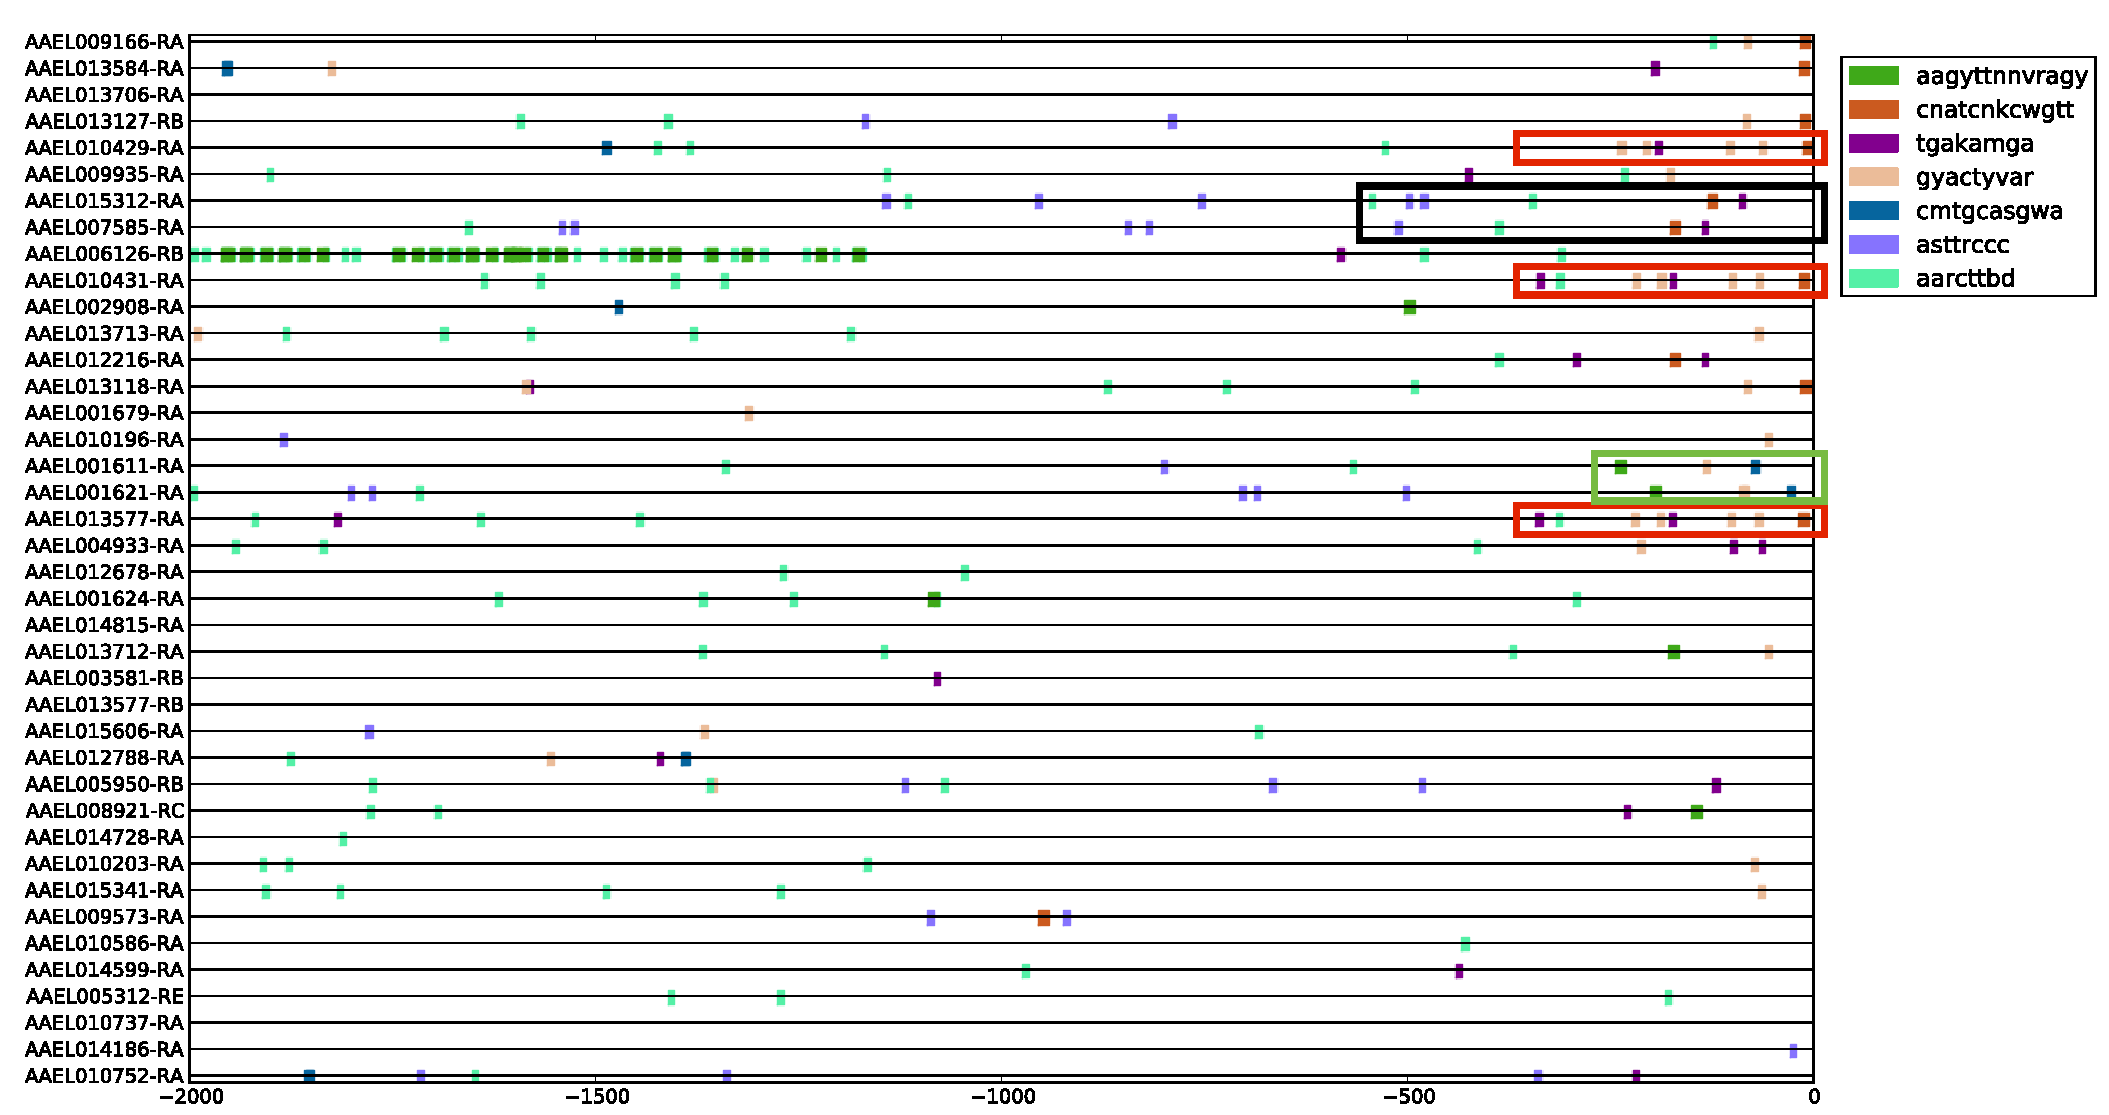
\includegraphics[width=.99\textwidth]{figures/figs/bonizzoni2011-cres.pdf}

\caption[Motif map of putative CREs from transcripts detected only in bloodfed female \Aa]{\sf \textbf{Motif map of putative CREs discovered by SCOPE using transcripts detected significantly only in bloodfed female \Aa:} Locations of representative SCOPE-derived CRE motifs in the 2000 bp upstream of the annotated translational start site in the 40 transcripts detected significantly only in bloodfed females. Transcript names on the left are ordered from most (top) to least (bottom) abundant.  Candidate CRMs are highlighted in like-colored rectangles.

Adapted from \cite{Bonizzoni2011}}
\label{fig:bonizzoni2011-cres}
\end{figure}
\begin{table}[hp]
 \begin{center} \sf
\begin{tabular}{cc}\toprule
\textbf{Distance from annotation (bp)} & \textbf{Predicted junctions}\\ \midrule
0-1000 & 1170\\
1001-2000 & 120\\
2001-4000 & 149\\
4001-8000 & 245\\
8001-16000 & 486\\
16001-32000 & 517\\
> 32000 & 854\\ \midrule
\textbf{Total} & \textbf{3541}\\ \bottomrule
 \end{tabular}
 \end{center}

\caption[Predicted novel junctions within various symmetric distance-windows from annotated transcripts]{\sf \textbf{Predicted novel junctions within various symmetric distance-windows from annotated transcripts:} \\
(Gene build AaegL1.2)\\
Excerpted from \cite{Bonizzoni2011}}

\label{tab:bonizzoni2011-novel-junx}
\end{table} 


% [-17] Brackney2010
% [-31] Fischer2008
% [-32] Pane2007
% [-33] Lawson2009
% [-50] Salazar2007
% [-54] Marelli2006
% [-55] Amenya2010
% [-56] Carlson2007
% [-57] Kriventseva2008
% [-58] Sieglaff2009
% [-60] Hubbard2002
% [-61] GENEBUILD?
% [-62] Bennet2002
% [-63] Black2002
% [-64] Terenius2008



Bonizzoni and Dunn \cite{Bonizzoni2011} provides a detailed examination of the changes in transcripts accumulation occurring at the whole-body level of \Aa\  females 5 hours \gls{PBM}. The observed changes are consistent with the beginning of an intense physiological response to a bloodmeal. The majority of immunity-related transcripts tended to accumulate at lower levels in blood fed mosquitoes. This finding supports the hypothesis that there may be a gap in immunity following a bloodmeal. Reduced expression of immune genes in blood fed mosquitoes could favor the establishment of infections, especially considering that pathogens such as dengue viruses infect the midgut epithelial cells within minutes after the contact \cite{Salazar2007}. However, changes in transcript abundance observed at the whole-body level may mask changes in accumulation occurring primarily in the midgut. Different levels of activation of immunity genes after a blood feeding may be one of the factors contributing to the variability in vector competence for dengue viruses observed in different geographic populations of \Aa\  \cite{Bennet2002,Black2002}. The quantity and quality of data generated by RNA-seq technology makes this an ideal approach for comparative analyses of the transcriptome of \Aa\ strains with different vector competence and vectorial capacity.

Our analyses of the expression profiles of sugar-fed (S) and bloodfed (B) mosquitoes allowed the identification of co-regulated genes and putative \textit{cis}-regulatory elements and modules from the \Aa\  genome. Further knowledge of the mechanisms involved in regulation of gene expression in vector species is critical to the development of control strategies whereby the vector is modified genetically to express anti-pathogen effector molecules in tissue-specific and time-regulated manners \cite{Terenius2008}. Promoter and other \textit{cis}-acting regulatory DNA fragments are needed to regulate restricted expression of selected anti-pathogen effector molecules. Moreover, we described several examples of how the RNA-seq data generated can help improve the current annotation of the \Aa\  genome.

\subsection{Transcripts found exclusively in bloodfed mosquitoes}
Forty transcripts were found only in bloodfed mosquitoes, with the highest read-counts reaching ~1000/transcript, after normalizing for different library sizes (data not shown). Functional parent attribution for these transcripts is consistent with a role in digestion and in the progression of the gonotrophic cycle. Specifically, two transcripts, Aa5G1 (AAE013712-RA) and AaSPVI (AAE010196-RA), correspond to the midgut serine proteases shown previously to be elicited by a bloodmeal in the midgut of \Aa\  females \cite{Brackney2010}. Seven other transcripts encode enzymes (i.e. decarboxylase, cathepsin b and trypsins), and two are implicated in trafficking. Transcripts AAE014815-RA and AAE005950-RB correspond to the vacuolar protein sorting 13B from yeast and the chloride channel protein 2, respectively. Ten transcripts are paralogous to the G12 gene of \Ag\ and share the Insect Allergen Repeat motif. This motif is hypothesized to be a novel, insect-specific detoxifying domain implicated in the co-evolution of herbivorous insects and their plant hosts and also has been linked to nitrile-specific detoxification \cite{Fischer2008}. Transcripts AAEL006126-RB and AAEL008921-RC are predicted orthologues of the \Cxq\ vitellogenin-A1 gene and the \Dmel\ spaghetti squash (sqh) gene, respectively. The sqh gene product encodes the regulatory light-chain of non-muscle myosin II, which is required for cytoplasmic transport in nurse cells during oogenesis and also has been implicated in germline \gls{RNAi} processes \cite{Pane2007}.

\subsection{\textit{Cis}-regulatory element discovery}
Tightly regulated and bloodmeal-induced expression profiles are of particular interest for designing transgenic mosquito-based control strategies to reduce transmission of dengue fever. \textit{Cis}-regulatory sequences derived from bloodmeal-induced/up-regulated mosquito genes allow potentiating swift induction and effective levels of transcription of an associated effector gene, while likely inflicting the least fitness cost \cite{Marelli2006,Marelli2006}. We interpret the different levels of mRNA accumulation seen in this study to reflect changes in transcriptional activity of the corresponding genes, although it is possible that some levels may vary as a function of changing transcript stability or rates of turnover. With this in mind, we used SCOPE \cite{Carlson2007} to predict putative \glspl{CRE} that may provide the basis for rational identification and selection of new candidate promoter regions and for modification of the transcriptional profiles of current transgene constructs. We examined the 2000 base pairs (bp) flanking the 5'-boundaries of the 40 transcripts that were undetected in libraries from sugar-fed mosquitoes but detected at significant levels in the RNA-seq libraries from bloodfed mosquitoes and identified a redundant list of 22 motifs that are enriched significantly in these sequences \ref{fig:bonizzoni2011-cres}. A possible \gls{CRM} constructed with the discovered \glspl{CRE} is represented by the motif consensus sequences, cnatcnkcwgtt, gyactyvar, and tgakamga, and is associated with \Aa\  paralogues of the G12 gene of \Ag\ (AGAP006187) \ref{fig:bonizzoni2011-cres}. \Aa\ has 17 G12 genes, many more relative to other insects, which have 4.5 on average (according to OrthoDB; group EOG95TCTG) \cite{Kriventseva2008}. The transcripts of nine of the G12 paralogues are present in this co-regulated gene set (representing ~25\% of the 40).

Another putative \gls{CRM} contains the consensus sequence tgakamga, cnatcnkcwgtt, asttrccc and aarcttbd \ref{fig:bonizzoni2011-cres}. This \gls{CRM} groups with the cathepsin b genes, AAEL015312-RA and AAEL007585-RA. Verification of these \glspl{CRM} will require empirical testing, however, the top 10 matches for tgakamga, which is present in both putative \glspl{CRM}, align well to members of the mosquito-conserved GATA motifs correlated to transcriptional responses to blood feeding in \Ag\ \cite{Sieglaff2009}.





\subsection{RNA-seq identifies annotation corrections}
RNA-seq also provides an opportunity to examine and improve the current annotation of the \Aa\  genome and examine the level of transcriptome plasticity in terms of alternative splicing. We used HMMSplicer \cite{Sieglaff2009} to compare junctions revealed by our data to the annotation provided by Vectorbase and Ensembl \cite{Lawson2009,Hubbard2002}. HMMSplicer predicted 32,501 junctions supported by at least two RNA-seq reads using the combined data from sugar and bloodfed samples. Of these, 24,100 (74\%) matched junctions present in the AaegL1.2 gene-build provided by VectorBase, leaving 8,401 predicted novel high-scoring splice sites supported by multiple RNA-seq reads. A total of 4500 (~54\%) of these occur within annotated gene boundaries and may represent un-annotated alternatively-spliced transcripts. To estimate how many of the remaining splice junctions might be truly novel, we mapped them to increasingly larger DNA fragments flanking the currently-annotated genes (Table \ref{tab:bonizzoni2011-novel-junx}). A total of 2687 (~33\%) junctions mapped within 32,000 bp of the 5'- or 3'-ends of annotated gene boundaries. Of these, 1439 mapped within 4000 bp, consistent with the interpretation that they may represent alternatively-spliced transcripts of the previously-identified genes. Those mapping beyond 4000 bp could be alternate junctions of the known genes, represent un-annotated transcription products or be artifacts.


An accurate gene annotation, especially with respect to the \gls{TSS}, is considerably advantageous with respect to the accurate discovery of \glspl{CRE} because prediction tools must make the assumption that the sequences included are true regulatory regions, and their performance suffers when this is false. For the \gls{CRE} predictions described in the previous section, 36 of the 40 transcript start sites were in close agreement to the Ensembl annotation \cite{Hubbard2002}. Figure \ref{fig:aedesHMMsplice} highlights three determined amendments to the current annotation, all supported by EST data. Figure \ref{fig:aedesHMMsplice} (A and B) supports the conclusion that the current annotation has missed the putative first exons that extend the 5'-UTRs of some genes (AAEL006259, AAEL010818) and provides additional information for predicting accurate \glspl{TSS}. In the case of AAEL010818, the \gls{TSS} determined by RNA-seq data is 20 kb to the 5'-end of the annotated start site, far outside the distances commonly searched for \glspl{CRE} (Figure \ref{fig:aedesHMMsplice} B). In some cases, as was seen for AAEL001774, the first exon was annotated but included as a separate gene model, which also contains the likely 5'-UTR of AAEL001759 (Figure \ref{fig:aedesHMMsplice} C). AAEL001774 encodes a protein comprising 50 amino acids with no known functional domains aside from a predicted signal peptide that makes up 66\% of its length.

